\RequirePackage{amsmath}
\documentclass[twocolumn, times]{aastex63}
\usepackage[spanish,es-minimal,english]{babel}
\usepackage[utf8]{inputenc}
\usepackage{natbib}
%\usepackage{microtype}
\usepackage{hyperref}
\usepackage{savesym}
\savesymbol{tablenum}
\usepackage{siunitx}
\restoresymbol{SIX}{tablenum}
\usepackage[varg]{newtxmath}
\usepackage{newtxtext}
\usepackage{booktabs}
\usepackage{array}   % for \newcolumntype macro
\newcolumntype{L}{>{$}l<{$}} % math-mode version of lrc column types
\newcolumntype{R}{>{$}r<{$}} 
\newcolumntype{C}{>{$}c<{$}} 

\bibliographystyle{aasjournal}

\sisetup{
  % explicit""+" is useful for velocities
  retain-explicit-plus = true,
  % prefer 10^6 over 1 x 10^6
  retain-unity-mantissa = false,
}

% A better \ion command that works in more circumstances
\newcommand\ION[2]{#1\,\scalebox{0.9}[0.8]{\uppercase{#2}}}
\newcounter{ionstage}
\renewcommand{\ion}[2]{\setcounter{ionstage}{#2}% 
  \ensuremath{\mathrm{#1\,\scriptstyle\Roman{ionstage}}}}
\newcommand\hii{\ion{H}{2}}

% Stars in Orion, e.g., \th1C, \th2A
\def\th#1#2{\(\theta^{#1}\)\,Ori~#2}
% Wavenumbers
\newcommand\wn{\ensuremath{\tilde{\nu}}}

% Chemical formulae
\newcommand*\chem[1]{\ensuremath{\mathrm{#1}}}
% Atomic term symbols
\newcommand\Config[1]{\ensuremath{\mathrm{#1}}}
\newcommand\Term[3]{\ensuremath{\mathrm{#1\ ^{#2}#3}}}
\newcommand\Level[4]{\ensuremath{\mathrm{#1\ ^{#2}#3_{#4}}}}

% Emission lines
\newcommand\ha{\ensuremath{\text{H}\alpha}}
\newcommand\lya{\ensuremath{\text{Ly}\alpha}}
\newcommand\lyb{\ensuremath{\text{Ly}\beta}}
\newcommand\Raman{\ensuremath{_{\text{Raman}}}}

\begin{document}
%\title{Raman mapping of atomic hydrogen and oxygen in the Orion Bar and Orion South PDRs}
\title{Raman mapping of photodissociation regions in Orion}
\shorttitle{Raman mapping of Orion PDRs}
\author{William J. Henney}
\affiliation{%
  \foreignlanguage{spanish}{Instituto de Radioastronomía y
    Astrofísica, Universidad Nacional Autónoma de México, Apartado
    Postal 3-72, 58090 Morelia, Michaoacán, Mexico}}
\email{w.henney@irya.unam.mx}

\begin{abstract}
  I show that the broad Raman-scattered wings of H\(\alpha\) can be used to
  map neutral gas illuminated by high-mass stars in star forming
  regions. The near wings
  (\(\Delta\lambda \approx \pm \SI{10}{\angstrom}\)) trace neutral hydrogen columns of
  about \SI{5e20}{cm^{-2}}, while the farther wings
  (\(|\Delta\lambda| > \SI{30}{\angstrom}\)) trace columns of about
  \SI{5e21}{cm^{-2}}. Absorption features in the pseudo-continuum at
  6633 and 6664~\AA{} correspond to neutral oxygen far-ultraviolet
  absorption lines at \SIlist{1027.43;1028.16}{\angstrom}.
\end{abstract}

\keywords{Atomic physics; Radiative transfer; Photodissociation regions}
\facilities{VLT:Yepun (MUSE); OANSPM:2.1m (Mezcal); Keck (HIRES)}
%\object{M42}
\section{Introduction}
\label{sec:introduction}

Raman scattering is the inelastic analog of Rayleigh scattering by
atoms or molecules.  Both processes begin with a radiation-induced
transition of an electron to a virtual bound state (non-eigenstate).
In Rayleigh scattering, the electron returns to its original state,
resulting in the radiation being re-emitted with its original
frequency (elastic scattering).  In Raman scattering, on the other
hand, the electron undergoes a transition to a different excited
state, resulting in radiation being re-emitted at a much lower
frequency.  Recently, \citet{Dopita:2016a} identified exceedingly
broad wings to the \ha{} \SI{6563}{\angstrom} line in the Orion Nebula
and a number of \hii{} regions in the Magellanic Clouds, which they
ascribe to Raman scattering of ultraviolet radiation in the vicinity
of the \lyb{} \SI{1025}{\angstrom} transition.  Raman scattering in
astrophysical sources was first identified in symbiotic stars
\citep{Schmid:1989a}, where FUV \ion{O}{6} emission lines at
\num{1032} and \SI{1038}{\angstrom} produce broad emission features at
\num{6827} and \SI{7088}{\angstrom}.  This illustrates a curious
feature of Raman scattering \citep{Nussbaumer:1989a}: the relative
width \(\Delta\lambda/\lambda\) of spectral features is amplified by a factor
\(\lambda(\ha)/\lambda(\lyb) \approx 6.4\) when passing from the FUV to the optical
domain.

\citet{Dopita:2016a} propose that the Raman wings form at the
transition zone near the ionization fronts in \hii{} regions.
However, the total neutral hydrogen column through the ionization
front can be no more than about
\(10 / \sigma_0 \approx \SI{2e18}{cm^{-2}}\), where
\(\sigma_0 \approx \SI{6.3e-18}{cm^2}\) is the ground-state hydrogen
photoionization cross section at threshold \citep{Osterbrock:2006a}.
The Raman scattering cross section at wavelengths responsible for the
observed wings is much lower than this:
\(\sigma\Raman \sim \SI{e-21}{cm^2}\) \citep{Chang:2015a}, meaning that the
Raman scattering optical depth through the ionization front is only of
order \(0.001\).  A vastly larger column density of neutral hydrogen
(\(\approx \SI{e21}{cm^{-2}}\)) is available in the photodissociation region
(PDR) outside the ionization front, so it is more likely that Raman
scattering will occur there instead, so long as there is sufficient
far ultraviolet radiative flux.

This paper is organized as follows. \S~\ref{sec:raman-theory}
recapitulates the basic theory of Raman scattering, concentrating on
the wavelength transformation from the FUV domain around \lyb{} to
optical domain around \ha{}.  In addition, polynomial fits are
provided to the wavelength dependence of the total (Rayleigh plus
Raman) scattering cross section and the Raman \ha{} branching
ratio. \S~\ref{sec:muse-spectr-mapp} then presents archival VLT-MUSE
integral field spectroscopy of the Orion Nebula, which allows the
broad H\(\alpha\) wings to be spatially mapped in unprecedented detail and
compared with other tracers of ionized and neutral zones in the
nebula.  Two components of the \ion{O}{1} UV resonance multiplet
\(\Term{2p^4}{3}{P} \to \Term{3d}{3}{D^o}\) are detected as absorption
features at \num{6633} and \SI{6664}{\angstrom} against the \ha{}
Raman wings.  \S~\ref{sec:keck-observations} presents archival
Keck-HIRES slit spectroscopy, which shows the profile of the
\SI{6664}{\angstrom} absorption line with an effective velocity
resolution of \SI{1}{km.s^{-1}}.  \S~\ref{sec:discussion} discusses
the implications of these results for the structure and dynamics of
the PDRs in Orion, together with the prospects for using Raman
spectral mapping as a diagnostic tool in the study of other high-mass
star formation regions.

\section{Raman scattering theory}
\label{sec:raman-theory}

\begin{table*}
  \caption{FUV/optical wavelength equivalencies for Raman scattering}
  \label{tab:raman-wavelengths}
  ~\\[-\baselineskip]
  \begin{tabular}{L L L C C R C C C}\toprule
    % Transition & {UV wav, \AA{}} & {Freq, cm\textsuperscript{-1}} & {d Freq} & {Opt wav} & {Air wav}\\
    \text{Ion} & \text{Transition} & J_i \to J_k & \lambda_1,\ \si{\angstrom} & \wn_1,\ \si{cm^{-1}} & \Delta\wn,\  \si{cm^{-1}}& \wn_2,\ \si{cm^{-1}} & \lambda_2,\ \si{\angstrom} & \lambda_{\text{air}},\ \si{\angstrom} \\
    \midrule
    & & & \multicolumn{2}{c}{\dotfill\(\quad \lyb,\ n = 1 \quad\)\dotfill} & & \multicolumn{3}{c}{\dotfill\(\quad \ha,\ n = 2 \quad\)\dotfill} \\
    \addlinespace[2pt]
    \ion{H}{1} & n\Term{s}{2}{S} \to \Term{3p}{2}{P} & \tfrac12 \to \tfrac12,\tfrac32 & 1025.72220 & 97492.283 & 0.000 & 15233.329 & 6564.553 & 6562.740\\
    \addlinespace
    \ion{O}{1} & \Term{2s^2 2p^4}{3}{P}  \to \Term{2s^2 2p^3 (^4S) 3d}{3}{D^o} & 0 \to 1 & 1028.15729 & 97261.383 & -230.900 & 15002.429 & 6665.587 & 6663.747\\
     & & 1 \to 1 & 1027.43139 & 97330.100 & -162.183 & 15071.146 & 6635.196 & 6633.364\\
     & & 1 \to 2 & 1027.43077 & 97330.159 & -162.124 & 15071.205 & 6635.170 & 6633.338\\
     & & 2 \to 1 & 1025.76339 & 97488.369 & -3.914 & 15229.415 & 6566.240 & 6564.427\\
     & & 2 \to 2 & 1025.76276 & 97488.429 & -3.854 & 15229.475 & 6566.215 & 6564.401\\
     & & 2 \to 3 & 1025.76170 & 97488.530 & -3.753 & 15229.576 & 6566.171 & 6564.358\\
    \bottomrule
  \end{tabular}
\end{table*}


When a photon is Raman-scattered from the vicinity of \lyb{} (UV
domain) to the vicinity of \ha{} (optical domain) its wavelength is
transformed from \(\lambda_1\) to \(\lambda_2\).  Intervals in frequency
(\(\nu = c/\lambda\)) or wavenumber (\(\wn = 1 / \lambda\)) space are conserved
between the two domains. For example the wavenumber displacement from
the \ion{H}{1} line center can be written in two ways:
\begin{equation}
  \label{eq:delta-wavnum}
  \Delta\wn = \wn_1 - \wn(\lyb) = \wn_2 - \wn(\ha) \ ,
\end{equation}
from which it follows that
\begin{equation}
  \label{eq:wav-transform}
  \lambda_2 = \left( \frac1{\lambda(\ha)} +\frac1{\lambda_1} - \frac1{\lambda(\lyb)}\right)^{-1} \ .
\end{equation}
The wavelengths \(\lambda(\lyb)\) and \(\lambda(\ha)\), together with their
corresponding wavenumbers, are given in
Table~\ref{tab:raman-wavelengths} (all wavelengths are on the vacuum
scale unless otherwise noted).  For both lines, a weighted average
over the \Level{3p}{2}{P}{1/2} and \Level{3p}{2}{P}{3/2} upper levels
is used, assumed to be populated according to their statistical
weights, with individual component wavelengths obtained from
Tab.~XXVIII of \citet{Mohr:2008a}. Note that the electric dipole
selection rules mean that only \Config{3p \to 2s} transitions contribute
to \ha{} in the Raman scattering context.  The wavelength is therefore
slightly shorter than the value obtained for the \ha{} recombination
line, which includes additional contributions from \Config{3s \to 2p}
and \Config{3d \to 2p}. The shift is of order \SI{-0.05}{\angstrom} or
\SI{-2}{km.s^{-1}} with respect to the Case~B results reported in
Tab.~6a of \citet{Clegg:1999a}.

Also listed in Table~\ref{tab:raman-wavelengths} are the Raman
transformations \(\lambda_1 \to \lambda_2\) for the rest wavelengths of transitions
between the ground \Term{2s^2 2p^4}{3}{P} term of neutral
\chem{^{16}O} and the excited \Term{2s^2 2p^3 3d}{3}{D^o} term. The
\ion{O}{1} data is obtained from highly accurate laser metrology
\citep{Ivanov:2008a, Marinov:2017a}, with a precision of
\SI{0.08}{cm^{-1}} or better.  The fine structure splitting between
the \(J_k\) levels of the excited term (\(\sim \SI{0.1}{cm^{-1}}\)) is
much smaller than that between the \(J_i\) levels of the ground term
(\(\sim \SI{100}{cm^{-2}}\)), so that the 6 transitions fall into 3
well-separated groups.  The three transitions from the lowest energy
\(J_i=2\) level are very close to \lyb{}
(\(\Delta\wn \approx \SI{4}{cm^{-1}}\)), whereas the two transitions from
\(J_i=1\) (\(\Delta\wn \approx \SI{162}{cm^{-1}}\)) and the single transition
from \(J_i=0\) (\(\Delta\wn \approx \SI{231}{cm^{-1}}\)) lie increasingly to the
red.  The corresponding wavelengths in the optical domain,
\(\lambda_2\), are therefore on the red side of \ha{}.  The final column of
the table uses STP refractive indices \citep{Greisen:2006a} to convert
\(\lambda_2\) to air wavelengths, \(\lambda_{\text{air}}\), for ease of comparison
with ground-based optical spectroscopy.  The resultant wavelength is
\SI{6663.747}{\angstrom} for the line from \(J_i = 0\), with an
uncertainty of about \SI{0.004}{\angstrom}, which is much smaller than
typical observational precision (for instance, \SI{0.07}{\angstrom}
for a very high resolution spectrograph with resolving power of
\(R = \num{e5}\)). The two lines from \(J_i = 1\), with a separation
of \SI{0.028}{\angstrom}, will always be blended in observations,
giving a mean wavelength of \SI{6633.347}{\angstrom} (assuming the
upper levels are distributed according to statistical weight
\(2 J_k + 1\)).  Similarly, the three lines from \(J_i = 2\) have a
mean wavelength of \SI{6564.386}{\angstrom}, but this is so close to
\ha{} (corresponding to a Doppler shift of \SI{+75}{km.s^{-1}}) that
it would be very difficult to observe.

The total cross-section for the off-resonance \Config{1s \to 3p}
transition in \chem{H^0} is calculated in \S~2 of \citet{Chang:2015a}
from second order time-dependent perturbation theory. Results are
presented in the upper panel of Figure~1 of that paper in terms of a
Doppler velocity factor \(\Delta V_1\), which in the notation of the
current paper is
\begin{equation}
  \label{eq:chang-DeltaV1}
  \Delta V_1 = c \left( \frac{\lambda_1}{\lambda(\lyb)} - 1 \right) \ .
\end{equation}
The observed Raman-scattered wings of \ha{} that are analyzed below
are typically within \(\Delta\lambda_2 \sim \pm \SI{100}{\angstrom}\) of the line
core.  It is therefore convenient to define a dimensionless wavelength
in the optical domain as
\begin{equation}
  \label{eq:x-optical-def}
  x = \frac{\lambda_2 - \lambda(\ha)}{\SI{100}{\angstrom}} \ ,
\end{equation}
which corresponds to \(x \approx \Delta V_1 / \SI{714}{km.s^{-1}}\) in the FUV
domain.  The total cross section in the range \(0.4 < |x| < 2.3\) can
then be fit as follows:
\begin{equation}
  \label{eq:total-cross-section-fit}
  \frac{\sigma}{\SI{e-21}{cm^2}} =  
  \begin{cases}
    0.2186 x^{-2} - 0.0344 x^{-1} - 0.0054 & \text{if \(x < 0\)} \\
    0.2367 x^{-2} - 0.0187 x^{-1} + 0.0041 & \text{if \(x > 0\)} 
  \end{cases}
\end{equation}
Note that separate fits are given for the blue (\(x < 0\)) and red
(\(x > 0\)) wings of \ha{} since the cross section, although
approximately Lorentzian, is not exactly symmetric, being stronger on
the blue side (by about 10\% for \(x = \pm 1\)).

The fraction of all \Config{1s \to 3p} excitations that result in Raman
scattering to an optical photon is given by the branching ratio,
\(f_{\ha}\), with the remaining fraction, \(1 - f_{\ha}\), resulting
in elastic Rayleigh scattering in which the photon remains in the FUV
domain.  The results for \(f_{\ha}\) are also shown in Figure~1 of
\citet{Chang:2015a} and can be fit as follows in the range
\(|x| < 5\):
\begin{equation}
  \label{eq:fha-fit}
  f_{\ha} = 0.2238 + 0.0363 x + 0.0024 x^2 \ .
\end{equation}
The relative accuracy of all these fits is better than 1\% within the
stated range (corresponding to
\(\sigma \approx \text{\SIrange{e-22}{e-21}{cm^2}}\)), which is perfectly
adequate for the purposes of this paper.  Note that the branching
ratio increases with \(x\), which means that the product
\(\sigma f_{\ha} \) is stronger on the red side of \ha{}.

\section{Spectral mapping of Raman wings}
\label{sec:muse-spectr-mapp}

\begin{figure}
  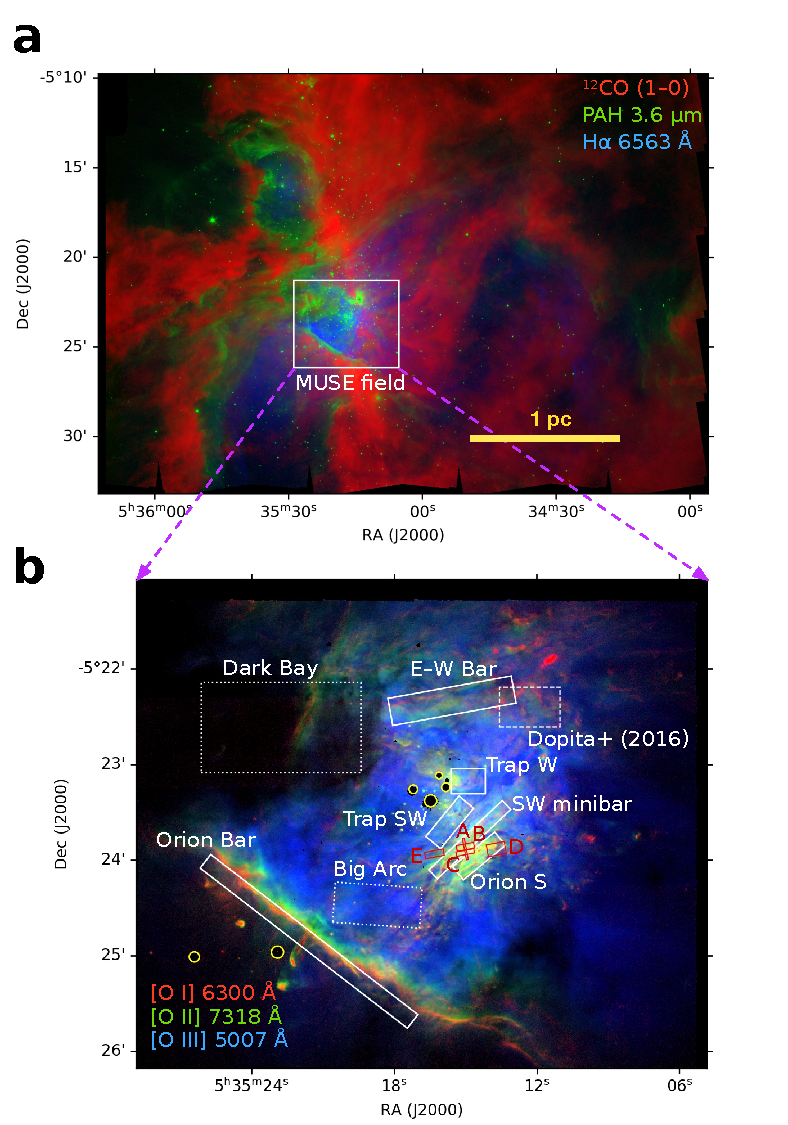
\includegraphics[width=\linewidth]{figs/raman-fov-regions}
  \caption{(a)~Panoramic view of the Orion Nebula region on parsec
    scales.  Red channel of background image shows \chem{^{18}CO}
    emission from dense molecular gas \citetext{Carma-NRO Orion
      Survey, \citealp{Kong:2018a}}. Green channel shows near-infrared
    continuum from PAH grains in neutral gas \citetext{Spitzer Orion
      Survey, \citealp{Megeath:2012a}}.  Blue channel shows optical
    H\(\alpha\) emission from ionized gas \citetext{WFI camera on ESO
      \SI{2.2}{m} La Silla, \citealp{Da-Rio:2009a}}. The white box
    shows the field of view observed with MUSE.  (b)~Locations within
    the nebula of the extraction regions for the MUSE spectra shown in
    Figure~\ref{fig:raman-spectra-1d} (white boxes) and the Keck HIRES
    spectra shown in Figure~\ref{fig:raman-keck} (red boxes).  The
    region of the spectrum obtained in \citet{Dopita:2016a} is shown
    by the dashed box. Background image shows oxygen emission lines
    extracted from the MUSE data cube: [\ion{O}{1}] \(\lambda6300\) (red
    channel), which traces ionization fronts and shocks in neutral
    gas; [\ion{O}{2}] \(\lambda7318\) (green channel), which traces the
    outer layers of the photoionized nebula; and [\ion{O}{3}]
    \(\lambda5007\) (blue channel), which traces the highly ionized interior
    of the nebula. }
  \label{fig:raman-fov-regions}
\end{figure}

\begin{table*}
  \caption{Wavelength bands used for Raman wing extraction}
  \label{tab:wav-bands}
  ~\\[-\baselineskip]
  \begin{tabular}{l l R C C C C l}\toprule
    & Band & \langle\Delta\lambda\rangle, \si{\angstrom}   & \lambda_{\text{min}}, \si{\angstrom} & \lambda_{\text{max}}, \si{\angstrom} & f_{\mathrm{H\alpha}} & \langle\sigma_\lambda\rangle, \SI{e-21}{cm^2} & Contamination \\
    \midrule
    Blue wing & B133 & -132.8& 6414.85& 6445.45 & 0.180 & 0.144 & \\
    & B080 & -79.5 & 6469.25& 6496.45 & 0.196 & 0.378 & Sky 6471, 6478\\
    & B054 & -53.6 & 6499.85& 6517.70 & 0.205 & 0.802 & \ion{O}{2}? 6502, 6510, Sky 6507\\
    & B033 & -32.8 & 6518.55& 6540.65 & 0.212 & 2.069 & [\ion{N}{2}] 6527.24, [\ion{Ni}{3}] 6533.76\\
    \addlinespace[2pt]
    Red wing & R040 & 40.3 &  6594.20& 6611.20 & 0.238 & 1.451 & Sky 6603\\
    & R058 & 57.7 &  6612.05& 6628.20 & 0.244 & 0.695 & \\
    & R087 & 87.1 &  6638.40& 6660.50 & 0.255 & 0.299 & [\ion{Cr}{4}]? 6641\\
    & R136 & 135.7 & 6688.55& 6708.95 & 0.274 & 0.119 & \ion{He}{1} 6699\\
    \bottomrule
  \end{tabular}
\end{table*}

\begin{figure*}
  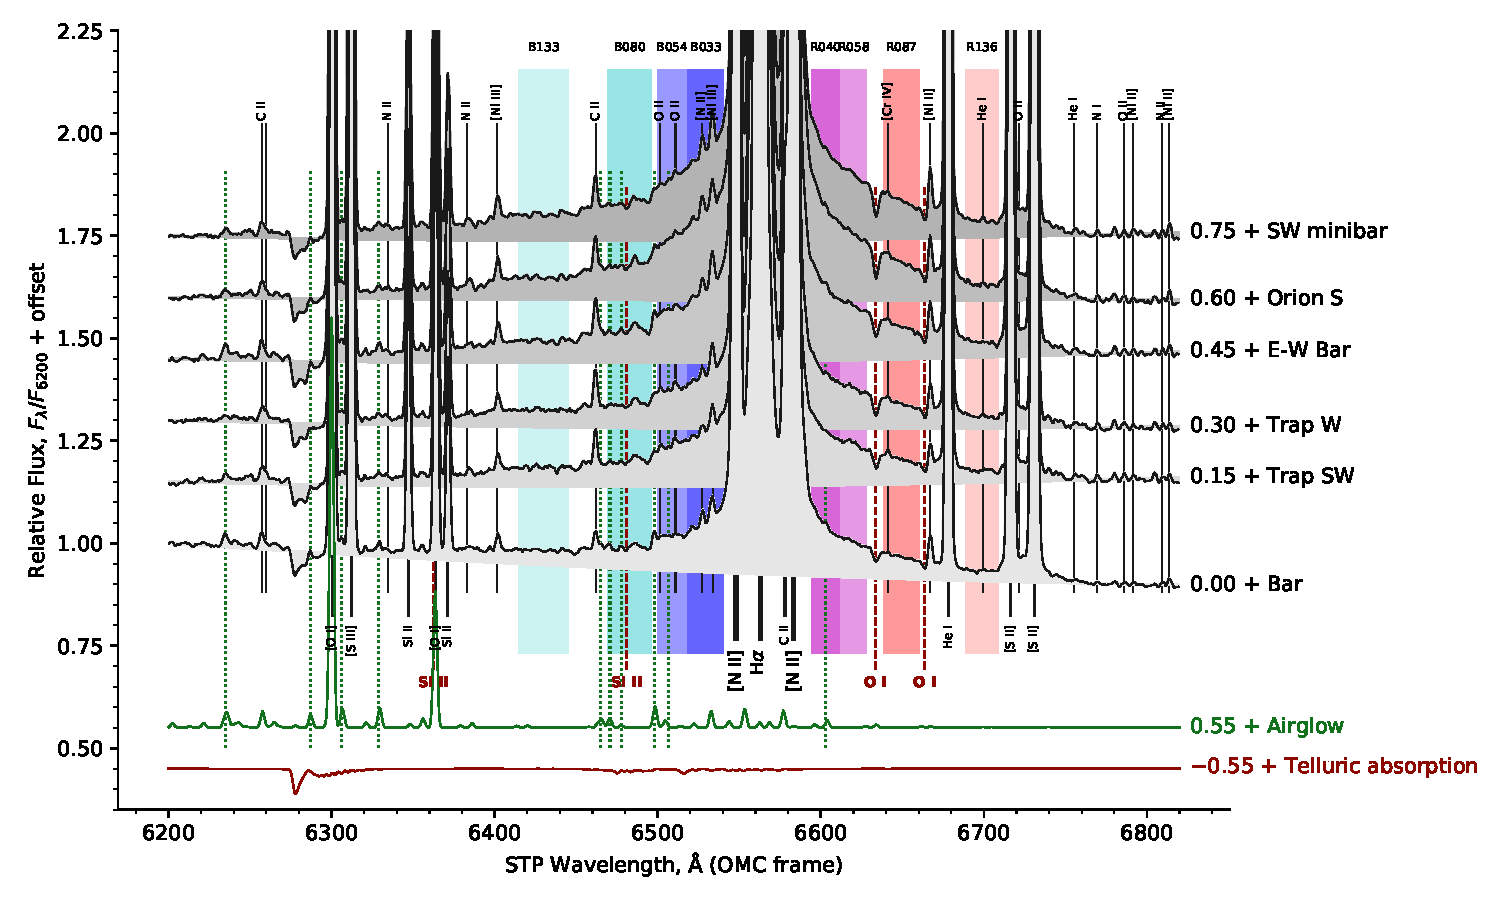
\includegraphics[width=\linewidth]{figs/raman-orion-muse-1d-spectra}
  \caption{MUSE spectra centered on the H\(\alpha\) line, showing the broad
    Raman-scattered wings.}
  \label{fig:raman-spectra-1d}
\end{figure*}

\begin{figure*}
  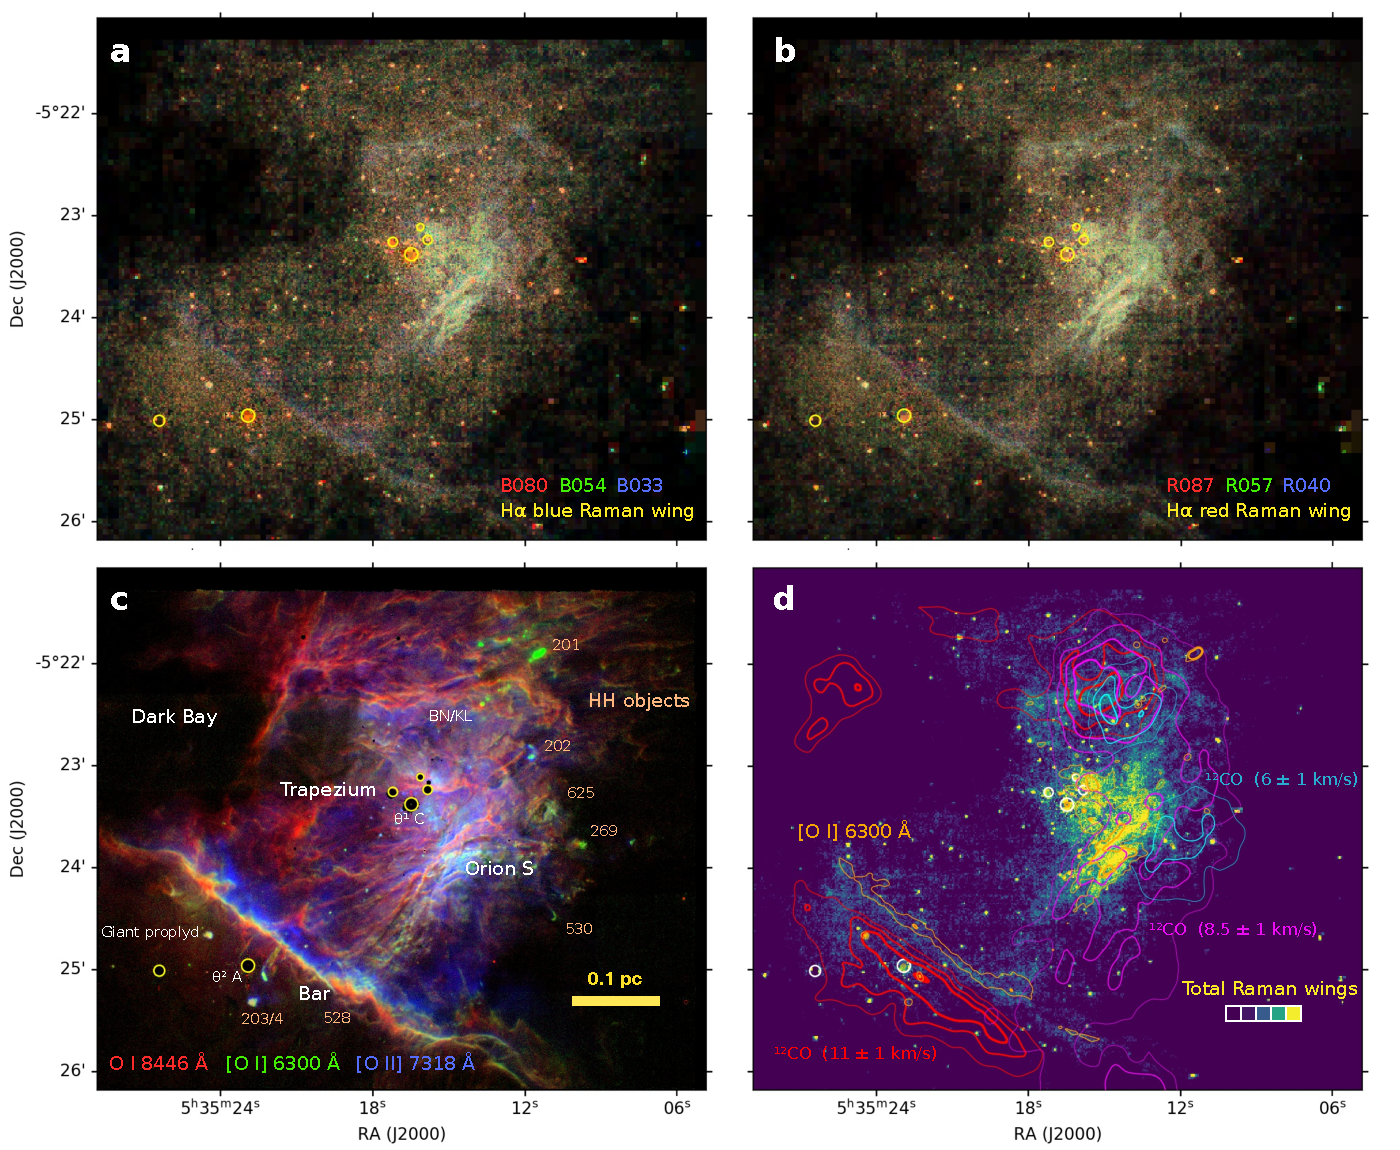
\includegraphics[width=\linewidth]{figs/raman-rgb-4-panel}
  \caption{Spatial distribution of Raman-scattered wings in H\(\alpha\)}
  \label{fig:raman-maps}
\end{figure*}

The \SI{6633}{\angstrom} and \SI{6664}{\angstrom} lines are clearly
detected in the MUSE spectra as absorption features against the
pseudo-continuum of the broad \ha{} wings (see Fig~XX), although the
latter is blended with a \ion{Ni}{2} emission line at
\SI{6666.8}{\angstrom}.  This is further proof of the Raman scattering
nature of the wings.




\begin{figure*}
  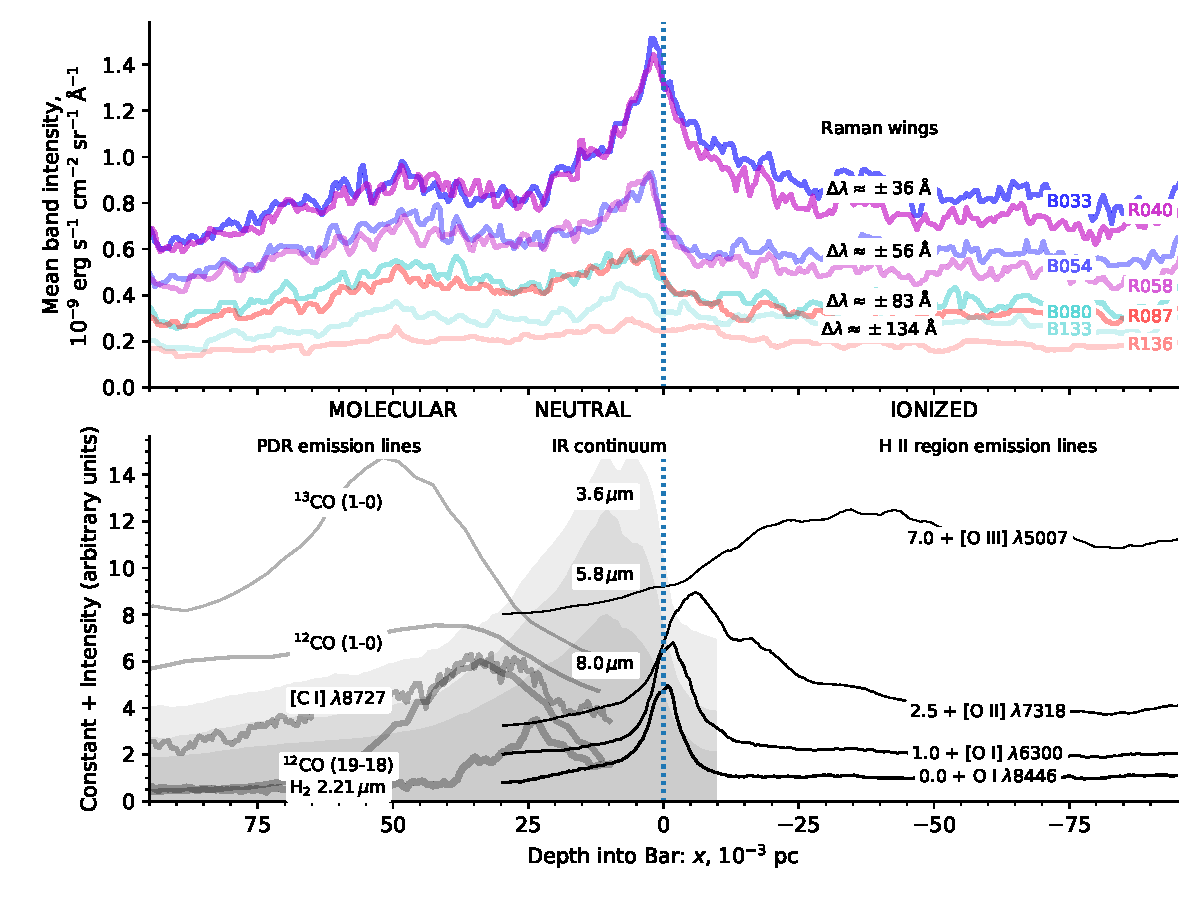
\includegraphics[width=\linewidth]{figs/raman-bar-multi-profile}
  \caption{Spatial cut of Raman-scattered H\(\alpha\) wing intensity across
    the Orion Bar (top panel). Matched red and blue wing bands are
    shown with color scheme matching
    Fig.~\ref{fig:raman-spectra-1d}. )}
  \label{fig:raman-bar-profile}
\end{figure*}

MUSE \citep{Bacon:2010a} observations of the Orion Nebula \citep{Weilbacher:2015a, Mc-Leod:2015b}.


The bands are chosen to avoid the stronger sky lines (e.g.,
\SI{6498}{\angstrom}) and nebula lines (e.g., ), but some weak line
contamination remains, as listed in the last column of
Table~\ref{tab:wav-bands}.


The 21~cm \ion{H}{1} line \citep{van-der-Werf:2013a} probes deeper
zones of the PDR than the Raman scattering, since it peaks at the
position of the \chem{H_2} emission.


\section{High-resolution spectroscopy of Raman-scattered \ion{O}{1} \SI{1028}{\angstrom}}
\label{sec:keck-observations}


Keck HIRES spectra described in \citet{Henney:1999a} and
\citet{Bally:2000a}. The spectrum I use is of HH~529 base region in
Orion~South. Published results from these data have concentrated on
strong nebular lines, but here I use a small section of the spectrum
in the range \SIrange{6660}{6670}{\angstrom} for reasons which will
become apparent.

\begin{figure}
  \includegraphics[width=\linewidth]{figs/raman-zoom-keck-regions}
  \caption{Zoom on Trapezium and Orion South region, showing regions
    of extracted Keck spectra.}
  \label{fig:zoom-keck}
\end{figure}

\begin{figure*}
  \centering
  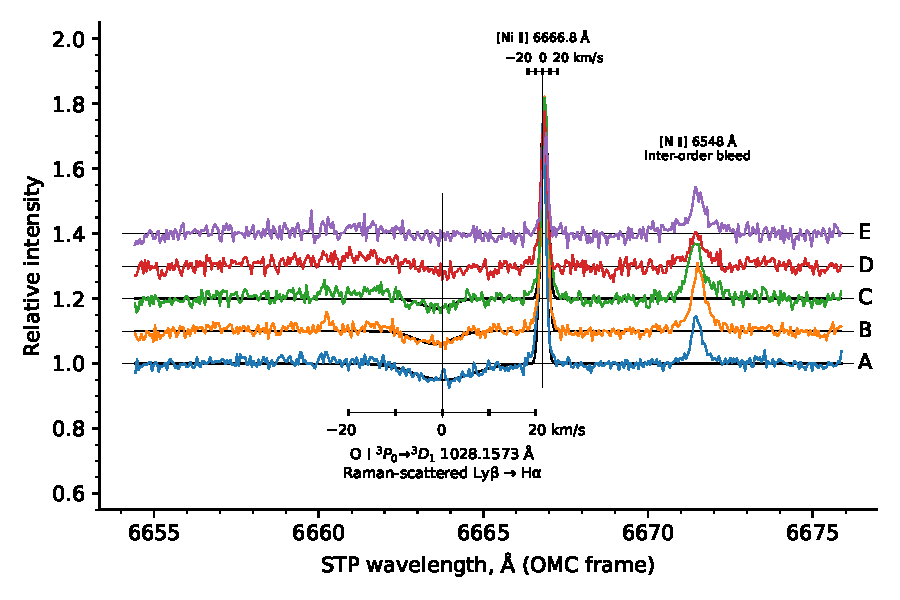
\includegraphics[width=\linewidth]{figs/order51-absorption-by-group}
  \caption{Keck HIRES spectra of Raman-scattered \ion{O}{1} absorption
    line for five regions in Orion~South.  Wavelengths are given on an
    air scale and in the rest-frame of the Orion Molecular Cloud, as
    defined by the peak velocity of \chem{^{13}CO}. }
  \label{fig:raman-keck}
\end{figure*}



\begin{table}
  \caption{Fit parameters from Gaussian line fits}
  \label{tab:line-fits}
  \begin{tabular}{l RRR RRR}\toprule
     & \multicolumn{3}{c}{\ion{O}{1}} & \multicolumn{3}{c}{\ion{Ni}{2}} \\
    Region & A & V & \sigma & A & V & \sigma \\ \midrule
    A & & & & & & \\
    B & & & & & &  \\
    C & & & & & &  \\
    D & & & & & &  \\
    E & & & & & &  \\ \bottomrule
  \end{tabular}
\end{table}

\section{Discussion}
\label{sec:discussion}

\begin{figure*}
  \centering
  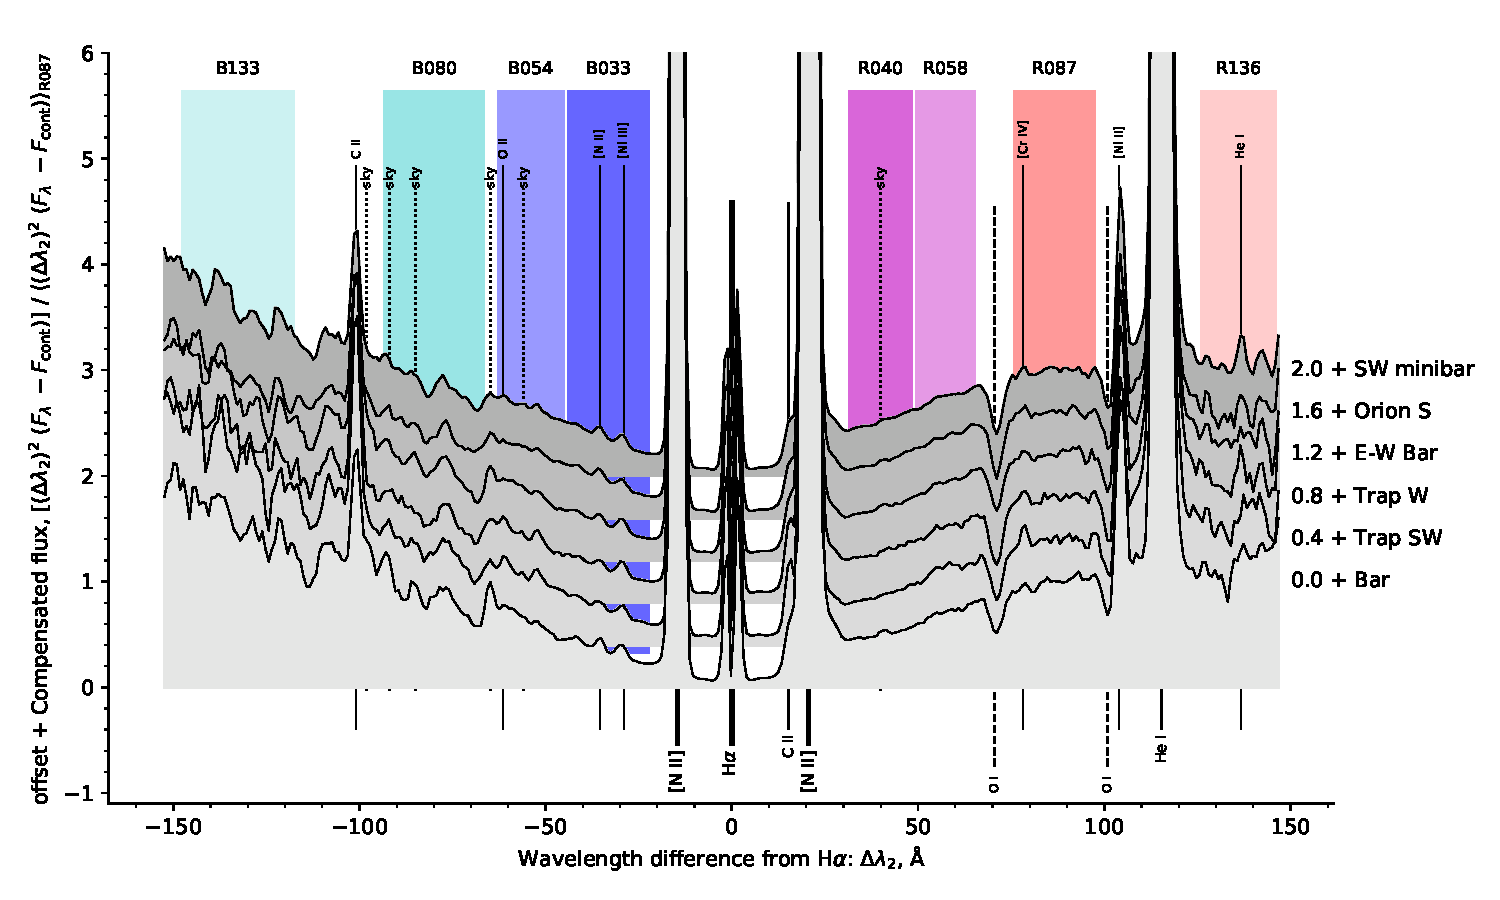
\includegraphics[width=\linewidth]{figs/raman-muse-spectra-times-lambda-squared}
  \caption{Same as Fig.~\ref{fig:raman-spectra-1d} but with
    \(F_\lambda\) multiplied by \((\Delta\lambda_2)^2\) and zoomed in on the Raman wing
    wavelengths.  The spectrum is normalized by the average flux in
    the R087 band and each region is offset vertically by a constant
    value, as indicated at right.  In this presentation, optically
    thin Raman scattering of a flat FUV spectrum should give a
    constant value, which for the Orion data is only seen in the R087
    and R136 bands.}
  \label{fig:raman-compensated}
\end{figure*}


Location of \chem{H^0}.  Neutral veil in front of nebula has column density of \SI{1.6e21}{cm^{-2}} and \SI{3.2e21}{cm^{-2}} in components A and B \citep{Abel:2006a}. 

\subsection{Structure of the Orion Bar}
\label{sec:structure-orion-bar}

Geometry of bar: in \citet{Henney:2005b} I pointed out that a
diverging cylindrical geometry is necessary to explain the sharp peak
in the [\ion{N}{2}] emissivity seen at the ionization front.  It has
been apparent since \citet{ODell:2000a} that the nebula contains many
bar-like features.

\citet{Salgado:2016a} had found low dust cross-section in Orion Bar
PDR, but there are loopholes. First, they assume plane-parallel
geometry with exactly edge-on viewing angle, while in reality it is a
roughly cylindrical filament.  Second, they ignore scattering, see
\citet{Watson:1998a}.  Also, density increase with depth

\begin{figure}
  \includegraphics[width=\linewidth]{figs/orion-bar-oi-hst-zoom}
  \caption{Fine-scale structure of the ionization front at the Orion Bar.}
  \label{fig:bar-oi-hst}
\end{figure}

\begin{figure}
  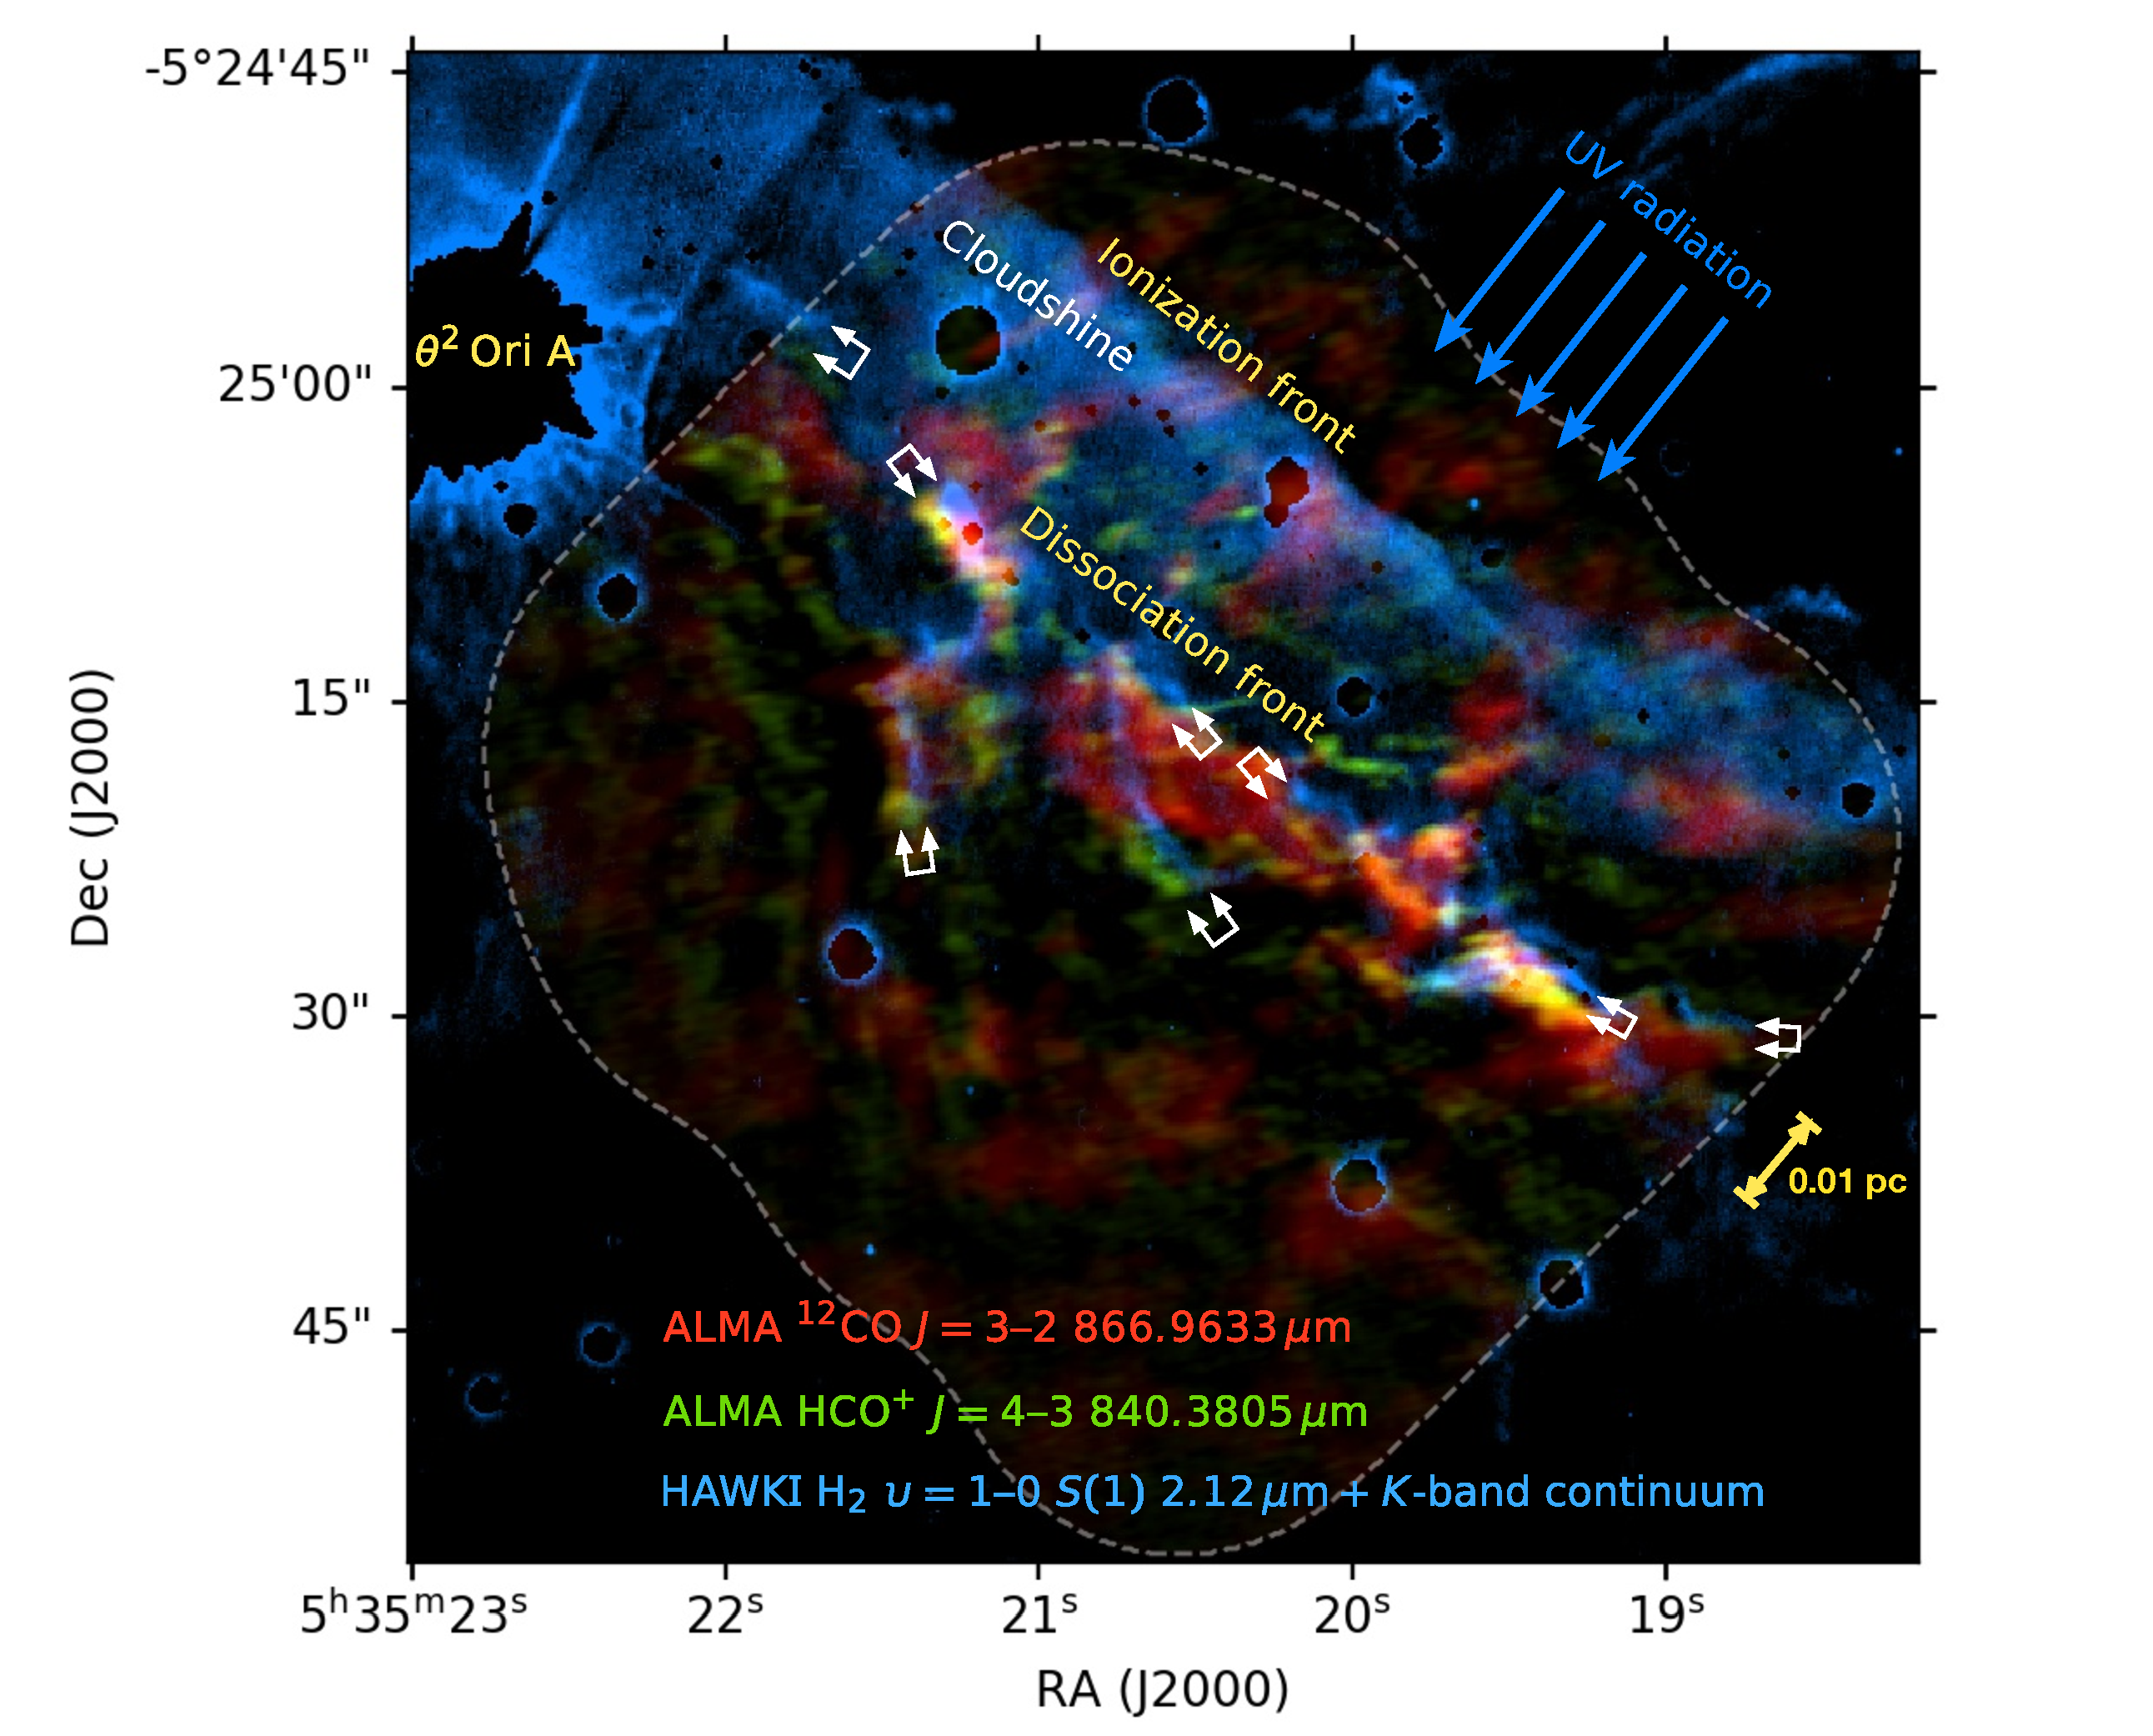
\includegraphics[width=\linewidth]{figs/alma-co-hcop-h2-dissoc-front}
  \caption{Fine-scale structure of the dissociation front in the Orion
    Bar.  Double white arrows mark out some instances of
    stratification between emission of \chem{H_2} (blue) and heavier
    molecules (green/yellow/red). In every instance \chem{H_2} is
    displaced towards the irradiated side of the filament by \(1''\)
    to \(2''\) (\(\approx \SI{0.003}{pc}\)).  Background image shows ALMA
    mosaics \citep{Goicoechea:2016a} of the sub-mm \chem{CO}
    \(J = 3 \to 2\) \SI{866.96}{\micron} \chem{HCO^+}
    \SI{840.38}{\micron} emission lines in the red and green color
    channels, respectively, with the boundary of the ALMA field shown
    by the gray dashed line. The blue color channel of the background
    image shows near-infrared vibrationally excited \chem{H_2}
    \(v = 1 \to 0\ S(1)\) \SI{2.12}{\micron} emission, extracted from
    narrow-band imaging with ESO's High Acuity Wide-field K-band
    Imager \citetext{HAWK-I, \citealp{Kissler-Patig:2008a}}. The
    \chem{H_2} image has been corrected for contamination by ionized
    emission (mainly hydrogen Br\(\gamma\) recombination line), but has not
    been continuum-subtracted.  As a result, scattered starlight
    \citetext{cloudshine, \citealp{Foster:2006a}} is seen as a band
    of diffuse emission that falls off smoothly behind the ionization
    front. }
  \label{fig:alma-dissoc-front}
\end{figure}

\subsection{Miscellany}
\label{sec:miscellany}



The effective resolving power of the optical spectrograph is multiplied by 6.4 for the FUV domain.

The \ion{O}{1} lines should be in absorption in the spectrum seen by the Raman scatterers. 

Non-equilibrium PDRs \citep{Stoerzer:1998a, Bertoldi:1996a}.  Recent models from \citet{Bron:2018a}. 

\ion{C}{1} emission from non-steady PDRs \citep{Stoerzer:1997a} (fine structure lines, but maybe optical lines would be similar).  \citet{Escalante:1991a} model the far-red [\ion{C}{1}] line as recombination of \chem{C^+}.


\ion{O}{6} 1037.62, 1031.93 absorption line in wind. No evidence for
a blue absorption edge at \(V = \SI{1200}{km.s^{-1}}\), which would be at
\(\lambda_2 = \SI{6649}{\angstrom}\), right in middle of R087 band.


Even for high PDR optical depth, no multiple Raman scattering will
occur since the population of \(2s\) is very small and the
post-scattered photons have insufficient energy to excite any
transitions from \(1s\).


\acknowledgments
This work has made use of the Atomic Line List\footnote{\url{https://www.pa.uky.edu/~peter/newpage/}} \citep{Van-Hoof:2018a}. 


\bibliography{BibdeskLibrary}

\appendix
\newcommand\vdw{vdW13}
\newcommand\vlsr{\ensuremath{v_{\mathrm{lsr}}}}
\section{Reanalysis of 21~cm \ion{H}{1} observations of the Orion Bar}
\label{sec:reanalysis-21-cm}

Karl G.\ Jansky Very Large Array observations of the \ion{H}{1}
\SI{21}{cm} line from the Orion Nebula and its surroundings at a
spatial resolution of \(\approx 6''\) and a velocity resolution of
\SI{0.77}{km.s^{-1}} were presented in \citet[hereafter
vdW13]{van-der-Werf:2013a}.  The line is seen both in emission and
absorption of the strong free-free continuum emitted by the ionized
nebula.  The majority of the absorption arises in the foreground Veil
at Local Standard of Rest velocities of
\(\vlsr = \text{\SIrange{-2}{+7}{km.s^{-1}}}\). Emission is seen
primarily at more redshifted velocities of
\SIrange{+10}{+15}{km.s^{-1}}, similar to the velocities of the
molecular gas seen in CO, although at large distances from the center
of the nebula the Veil is also seen in emission.  The analysis of the
absorption components by \vdw{} was carried out under the assumptions
that (i)~all of the continuum emission arises from \emph{behind} the
absorbing \chem{H^0} column (from the point of view of the Earth), and
(ii)~line emission is negligible at velocities where absorption is
detected.  These are both very good assumptions in the case of
absorption by the foreground Veil, but they break down for the case of
the Orion Bar, where both emission and absorption are seen at similar
velocities and in spatially adjacent regions.  Given the wealth of
information on the physical conditions and geometry that these data
provide, it is worth reanalyzing them under less restrictive
assumptions.

\newcommand{\Ttb}{\ensuremath{\tilde{T}_{\mathrm{b}}}}
\newcommand{\Tb}{\ensuremath{T_{\mathrm{b}}}}
\newcommand{\Tc}{\ensuremath{{T_{\mathrm{c}}}}}
\newcommand{\Te}{\ensuremath{T_{\mathrm{e}}}}
\newcommand{\Ts}{\ensuremath{T_{\mathrm{s}}}}

\begin{figure}
  \centering
  \caption{Three-layer sandwich structure for \ion{H}{1} \SI{21}{cm} radiative transfer.}
  \label{fig:hii-hi-hii-sandwich}
\end{figure}

In the Rayleigh--Jeans limit, the frequency-dependent surface
brightness \(I_\nu\) is characterized by the brightness temperature in
each velocity channel: \(T_{\mathrm{b}}(v) = c^2 I_\nu / 2 k \nu^2\),
where \(v/c = (\nu/\nu_0) - 1\) and \(\nu_0 = \SI{1.420405}{GHz}\).  The
radiative transfer equation can be solved for an idealized three-layer
sandwich structure (see Fig.~\ref{fig:hii-hi-hii-sandwich}),
consisting of (1)~a background \chem{H^+} region with electron
temperature \Te{} and free-free continuum optical depth \(\tau'\), (2)~an
intermediate neutral \chem{H^0} layer with spin temperature \Ts{} and
line optical depth \(\tau(v)\), and (3)~a foreground \chem{H^+} region
with the electron temperature \Te{} and free-free continuum optical
depth \(\tau''\). The continuum source function in regions~1 and~3 is
\Te{}, whereas the line source function in region~2 is \Ts{}.
Region~2 is assumed to have zero continuum optical depth.  Following
\vdw{}, large-scale Milky Way \ion{H}{1} line emission along the line
of sight through Orion is neglected since it is (a)~very faint
compared with the nebula, with \(\Tb(v) < \SI{48}{K} \) at
\(v = \SI{10}{km.s^{-1}}\) \citep{Green:1991a, Green:1993a}, and
(b)~any emission that is smooth on angular scales below 7 arcminutes
will be filtered out by the interferometer.
 
At continuum frequencies just off the line, \(\tau(v) = 0\) and only
regions~1 and 3 contribute to the observed brightness, yielding a
continuum brightness temperature
\begin{align}
  \label{eq:Tcont}
  \Tc & = \Te \biggl( 1 - e^{-(\tau' + \tau'')} \biggr) \\
  & = \Tc' e^{-\tau''} + \Tc''
  \ , \nonumber
\end{align}
where the second equality gives the decomposition into separate
contributions from region~1: \(\Tc' = \Te (1 - e^{-\tau'})\), and
region~3: \(\Tc'' = \Te (1 - e^{-\tau''})\).  At frequencies where the
line opacity is significant, all three regions contribute, yielding
\begin{equation}
  \label{eq:Tline}
  \Tb(v) =
    \Tc' e^{-\left(\tau(v) + \tau''\right)} +
    \Ts \biggl( 1 - e^{-\tau(v)} \biggr) e^{-\tau''} +
    \Tc''
  \ .
\end{equation}
For practical reasons related to the deconvolution of the
interferometric data, the results of \vdw{} are presented in
continuum-free form as \(\Ttb(v) = \Tb(v) - \Tc\).  Combining
equation~\eqref{eq:Tcont} and \eqref{eq:Tline}, one finds
\begin{equation}
  \label{eq:Tb}
  \Ttb(v) =
  \bigl[ 1 - e^{-\tau(v)} \bigr] \,
  \bigl[ 1 - \bigl(\Tc''/\Te\bigr)\bigr] \,
  \bigl[  \Ts - \Tc' \bigr]  \ .
\end{equation}
The relative brightness temperature of the line, \(\Ttb(v)\), is
therefore seen to be the product of three factors, given by the three
sets of square brackets in equation~\eqref{eq:Tb}.  The first two
factors are always positive since \(\tau(v) \ge 0\) and
\(\Tc'' \le \Te\), but the third factor can take either sign.  When the
continuum brightness temperature \(\Tc'\) of the background
photoionized gas in region~1 exceeds the spin temperature \(\Ts\) of
neutral hydrogen in region~2, then we see an absorption line:
\(\Ttb(v) < 0\).  On the other hand, when \(\Ts\) is higher than
\(\Tc'\), then we see an emission line: \(\Ttb(v) > 0\).  In either
case, the maximum line strength will be found when region~2 is opaque
(\(\tau(v) \gg 1\)) and region~3 is transparent (\(\Tc'' \ll \Te\)), yielding
\(\max(|\Ttb(v)|) = |\Ts - \Tc'|\).

\newcommand\fbg{\ensuremath{f_{\mathrm{bg}}}}

The electron temperature in the ionized gas is expected to be roughly
constant at \(\Te \approx \SI{11 000}{K}\) \citep{Dicker:2009a}, but this
still leaves 4 unknown quantities, \(\tau(v)\), \(\Ts\), \(\Tc'\), and
\(\Tc''\), to be determined from 2 observed quantities: \(\Tc\) and
\(\Ttb(v)\).  Further assumptions must therefore be made in order to
interpret the observations, but these can be guided by the observed
spatial trends and simple geometric models.  For instance, in the
Orion Bar the free-free continuum brightness temperature falls sharply
across the ionization front from \(\Tc \approx \SI{3000}{K}\) on the ionized
side, but then levels off to a roughly constant value of
\(\Tc \approx \SI{600}{K}\) on the neutral side. Assuming that this constant
value reflects unrelated foreground emission (probably ionized by
\th2{A}) that overlays the entire Bar (this hypothesis is tested
below), we have an upper limit to the background emission of
\(\Tc - \SI{600}{K}\).  It can be further assumed that the emission
from region~1 is a constant fraction, \fbg{}, of this upper limit:
\begin{equation}
  \label{eq:bg-emission}
  \Tc' = \fbg \bigl( \Tc - \SI{600}{K} \bigr) \ .
\end{equation}
If the Bar geometry is a cylinder that is illuminated from the side
(see Fig.~XXX), then \(\fbg = 0.5\) is appropriate.  If the Bar is
illuminated from slightly behind, or if it is an escarpment, or if an
additional background component is present (see
\S~\ref{sec:structure-orion-bar}), then the fraction will be larger:
\(0.5 < \fbg < 1.0\).

Further progress can then be made by considering null points in the
nebula where line emission and absorption cancel out. At such points
\(\Ttb(v) \approx 0\), so that \(\Ts = \Tc'\) by equation~\eqref{eq:Tb}.
Absorption component~M is identified by \vdw{} as associated with
\chem{H^0} in the Bar, due to its velocity and spatial distribution.
Component~M consists of a string of knots with
\(\Ttb(v) = \text{\num{-200} to \SI{-400}{K}}\) at
\(v \approx \SI{11}{km.s^{-1}}\).  They are arranged parallel to the Bar,
just behind the ionization front at a relative position of roughly
\SI{+0.006}{pc} (see Fig.~\ref{fig:raman-bar-profile}) and where the
continuum brightness has fallen to \(\Tc \approx \SI{2200}{K}\). At greater
distances from the ionization front the \ion{H}{1} at this velocity is
seen in emission, reaching a peak of \(\Ttb(v) \approx \SI{+250}{K}\) at
\SI{+0.030}{pc} where \(\Tc \approx \SI{750}{K}\).  The crossover null point
where \(\Ttb(v) = 0\) occurs between these two at \SI{+0.012}{pc}
where \(\Tc \approx \SI{1500}{K}\).

\textit{Add a table showing }

\end{document}
%%% Local Variables:
%%% mode: latex
%%% TeX-master: t
%%% End:
